% Created 2022-09-21 mié 19:56
% Intended LaTeX compiler: pdflatex
\documentclass[12pt]{article}
\usepackage[utf8]{inputenc}
\usepackage[T1]{fontenc}
\usepackage{graphicx}
\usepackage{grffile}
\usepackage{longtable}
\usepackage{wrapfig}
\usepackage{rotating}
\usepackage[normalem]{ulem}
\usepackage{amsmath}
\usepackage{textcomp}
\usepackage{amssymb}
\usepackage{capt-of}
\usepackage{hyperref}
\usepackage[spanish]{babel}
\usepackage{graphicx,geometry}
\geometry{ a4paper, left=1in, right=1in, top=1in, bottom=1in }
\renewcommand\familydefault{\sfdefault}
\usepackage{sectsty}
\sectionfont{\normalfont\Large }
\subsectionfont{\normalfont}
\usepackage{tabularx}
\usepackage{listings}
\lstdefinestyle{mystyle}{
numbers=left,
showspaces=false,
frame=leftline,
showspaces=false,
showstringspaces=false,
showtabs=false,
numberstyle=\tiny,
}
\lstset{
style=mystyle,
literate={á}{{\'a}}1
{é}{{\'e}}1
{í}{{\'{\i}}}1
{ó}{{\'o}}1
{ú}{{\'u}}1
{Á}{{\'A}}1
{É}{{\'E}}1
{Í}{{\'I}}1
{Ó}{{\'O}}1
{Ú}{{\'U}}1
{ü}{{\"u}}1
{Ü}{{\"U}}1
{ñ}{{\~n}}1
{Ñ}{{\~N}}1
{¿}{{?``}}1
{¡}{{!``}}1
}
\makeatletter
\usepackage{fancyhdr}
\pagestyle{fancy}
\usepackage{mdframed}
\BeforeBeginEnvironment{minted}{\begin{mdframed}}
\AfterEndEnvironment{minted}{\end{mdframed}}
\author{Luis Eduardo Galindo Amaya (1274895)}
\date{21-09-2022}
\title{Generación de un Programa Ejecutable}
\hypersetup{
 pdfauthor={Luis Eduardo Galindo Amaya (1274895)},
 pdftitle={Generación de un Programa Ejecutable},
 pdfkeywords={},
 pdfsubject={},
 pdfcreator={Emacs 26.3 (Org mode 9.1.9)}, 
 pdflang={Spanish}}
\begin{document}



\newcommand{\docente}{Arturo Arreola Alvarez}
\newcommand{\asignatura}{Organización de Computadoras (331)}
\newcommand{\semestre}{2022-2}

\newcommand{\miportada}[1]{
	\begin{titlepage}
		\vspace*{0.75in}
		\begin{flushleft}
			\sffamily
			\large #1       \\
			\Huge 
            \@title         \\
			\hrulefill
			\vspace{0.25in} \\
			\Large \@author \\
			\vspace*{\fill}
            
\includegraphics[width=\textwidth]{../includes/filler.png} \\
			\vspace*{\fill}
			\large
			\begin{tabular}{|l|l|}
              \hline
			  Asignatura & \asignatura \\
			  Docente    & \docente    \\
			  Fecha      & \@date      \\
              \hline
			\end{tabular}
		\end{flushleft}
	\end{titlepage}
}

\miportada{ Práctica 5 }

\fancyhf{}
\lhead{ \asignatura }
\rhead{ \semestre }
\rfoot{Página \thepage}

\setlength\parindent{0pt}   % eliminar el intentado
\setlength{\parskip}{1.2em}
\maketitle


\section*{Código}
\label{sec:orgfba8732}
\subsection*{codigo\_base.asm}
\label{sec:org26ddb9a}
\\ \lstinputlisting{./codigo_base.asm}

\subsection*{Compilando el Ejemplo}
\label{sec:orge6403eb}
\begin{verbatim}
nasm -f elf codigo_base.asm
ld -m elf_i386 codigo_base.o libpc_io.a -o salida.out
./salida.out 
\end{verbatim}

\begin{verbatim}
Hello, world!
\end{verbatim}

\pagebreak

\section*{Imprimir tres strings}
\label{sec:org24a4f4f}
Modificar código\_base.asm y nombrarlo Apellido\_Nombre\_P5.asm. Modificar el código para que imprima al menos 3 cadenas diferentes. Las cadenas debes ser definidas de la misma forma como se hace en código\_base.asm.

\\ \lstinputlisting{./Galindo_amaya_luis_eduardo.P5.asm}

\subsection*{Compilación}
\label{sec:orga4156cb}
\begin{verbatim}
nasm -f elf Galindo_Amaya_Luis_Eduardo.P5.asm
ld -m elf_i386 Galindo_Amaya_Luis_Eduardo.P5.o libpc_io.a -o salida2.out
./salida2.out 
\end{verbatim}

\begin{verbatim}
Hello, world!
Otro String!
y otro String!
\end{verbatim}

\pagebreak

\section*{Captura con getch y imprime con putchar}
\label{sec:orgda25ae3}
Dentro del mismo código, añada la opción de capturar un carácter (vea getche) y justo después, imprimirlo (vea putchar).

\\ \lstinputlisting{./captura-p5.asm}

\pagebreak

\section*{Conclusiones y dificultades}
\label{sec:orga20a190}
Nasm es mas difícil que marie.js, tiene operaciones mas avanzadas pero requiere que pongamos mas de nuestra parte para entender que estamos haciendo.

\section*{Capturas}
\label{sec:org1037ed7}
\begin{center}
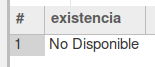
\includegraphics[width=.9\linewidth]{img/1.png}
\end{center}

\begin{center}
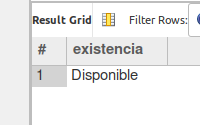
\includegraphics[width=.9\linewidth]{img/2.png}
\end{center}
\end{document}
